\chapter{Аналитические выражения}\label{ch:equations}
В данном разделе выполнены аналитические оценки для рассматриваемой задачи пробивания листа облаком осколков.
Оценки проведены по аналогии с пробитием бронежилетов пулями.
Важная особенность состоит в том, что существующие рассчёты проведены в иных скоростных режимах (скорость пули менее
1 $км/c$ ) и при существенно ином пространственном распределении нагрузки (массивный ударник, а не облако мелких
осколков).
Не смотря на это, после некоторой колибровки и сопоставления с экспериментом и численными рассчётами, результаты
аналитических вычислений можно использовать чтобы далее улучшить точность аналитических решений.

В этом разделе рассматривается композитный экран из множества слоёв ткани.
\section{Параметры}
Параметры волокон ткани приведены в \tabref{tbl:kevlar-params}

\begin{table}[h]
    \centering
    \caption{Параметры ткани}\label{tbl:kevlar-params}
    \begin{tabular}{|l|l|}
        \hline
        Параметр & Значение      \\ \hline
        Плотность & 1430 $кг/м^3$ \\ \hline
        Модуль Юнга & 125 ГПа       \\ \hline
        Предельное удлинение при разрыве & 4.25 \%       \\ \hline
        Прочность на разрыв & 4 ГПа         \\ \hline
        Прочность на сжатие & $40-60$ МПа     \\ \hline
    \end{tabular}
\end{table}

Данные по модулю Юнга, удлинению при разрыве, прочности на разрыв взяты из\cite{perepelkin2009,mikhailin2013}.
Значение прочности на сжатие взято, на основании данных\cite{papkov1986} о том, что прочность параамидных волокон
на сжатие $\approx 1.0 - 1.5 \%$ от прочности на растяжение.

Для пакета принимаем значение пористости: $\mu=0.6$\cite{buzov2004}.

Для облака частиц принимаем характерную скорость $v=4-6$ $км/с$.

\section{Этапы разрушения пакета}\label{sec:destr-stages}
Исходя из\cite{kobylkin2014} имеем три этапа столкновения ударника с пакетом:

Первый этап -- начало столкновения ударника с пакетом - уплотнение ударника в лицевой части,
ускорение материала в направлении движения ударника.
Разрушение нитей имеет сдвиговый характер.
Смещение слоёв мало.
Торможение ударника незначительно, так как этот этап имеет низкую продолжительность.

Второй этап -- проникновение ударника в пакет.
На этом этапе происходит растяжение и обрыв нитей.
Поперечное смещение велико, деформация превосходит предельную.
На этом этапе происходит торможение ударника и основное поглощение кинетической энергии.

Третий этап -- торможение ударника с образованием купола.
Поглощается оставшаяся часть кинетической энергии.

Для нашего скоростного режима имеет смысл обратить внимание на первые два этапа, так как ожидается полное пробитие пакета.

На начальном этапе столкновения в пакете возникает волна сжатия, в которой происходит поперечное движение слоёв ткани.
В задачах пробивания пакета массивный ударником (пулей) для оценки амплитуды волны сжатия рассматривается приближение,
в котором предполагается, что на фронте фолны происходит уплотнение до сплошного материала.
Воспользовавшись подходом, описаным в\cite{kobylkin2014}, предположим, что плотность изменяется скачком от некоторого
значения $\rho_0$ (с учётом плотности намотки нитей) до значения $\rho_m$ (плотность материала нитей).
\footnote{Следует обратить внимание, что этот приём не до конца обоснован в нашем случае, так как профиль удара сильно
отличается}

Очевидно, что при пористости $\mu$
\begin{equation}
    \rho_0 = (1 - \mu) \cdot \rho_m
\end{equation}
Что для нашего случая даёт: $\rho_m = 570~кг / м^3$

Применяя ЗСМ и ЗСИ для нашего пакета получим:
\begin{equation}
    \rho_0 D = \rho_m (D - u)
\end{equation}
\begin{equation}
    P = \rho_0 u D
\end{equation}
Здесь $D$ -- скорость фронта сжатия, а $u$ -- массовая скорость.

Получим:
\begin{equation}
    D = \frac{u}{\mu}
\end{equation}
\begin{equation}
    P = \frac{\rho_m (1 - \mu) u ^2}{\mu}
\end{equation}

Из этих оценок получаем, что уже при 2 $км/с$ давление будет 4 ГПа, что значительно больше чем прочность на сжатие.
С учётом принятой скорости в $4-6~км/с$ получим, данный процесс будет происходить по всей толщине пакета.

На основании теории\cite{rakhmatulin} и обших подходов и\cite{kobylkin2014} получим оценки для взаимодействия
осколка с нитями тканевого пакета.
При поперечном ударе по нити в ней начинают распространяться продольные и поперечные волны.
При взаимодействии частицы с тканевым пакетом зона высокого давления ограничена радиусом отрыва поперечной волны
в нитях ткани от поверхности частицы.
До отрыва поперечной волны от частицы общая конфигурация взаимодействия соответствует изображённой на
\picref{fig:first-stage}, а после - изображённой на \picref{fig:second-stage}

\begin{figure}[H]
    \centering

    \caption{Конфигурация до отрыва поперечной волны}
    \label{fig:first-stage}
    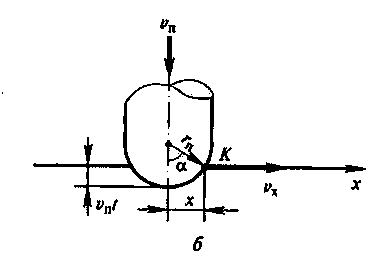
\includegraphics[width=0.5\textwidth]{img/first_stage.png}

    \caption{Конфигурация после отрыва поперечной волны}
    \label{fig:second-stage}
    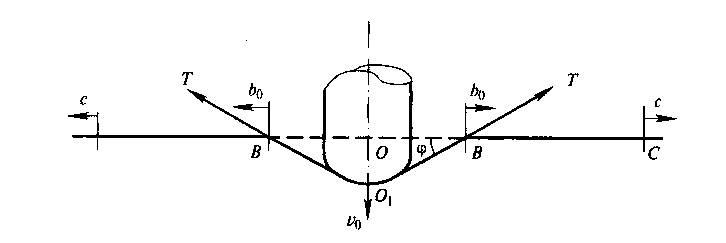
\includegraphics[width=0.8\textwidth]{img/second_stage.png}
\end{figure}

Для сферической частицы радиуса $r$, движущейся со скоростью $v$, скорость перемещения крайних точек контакта с
прямолинейной нитью, расположенной вдоль $Ox$, равна

\begin{equation}
    \frac{dx}{dt} = v_x = v \cdot \frac{r - v t}{\sqrt{r^2 - (r - v t)^2}}
\end{equation}

Для скорости поперечной волны в нити примем, для оценки, $c_s = v_a = 1~км/с$.

Обозначим радиус пятна контакта, при котором скорость достигнет $v_a$, через $r_a$.
Из геометрических соображений:

\begin{equation}
    \dfrac{r_a}{r} = \dfrac{1}{\sqrt{1 + (\dfrac{v_a}{v})^2}}
\end{equation}

Таким образом, для скорости $2~км/с$ радиус зоны высокого давления составляетс около $0.9$ радиуса частицы.
Для более высоких скоростей множитель стремится к единице.
Соответственно получаем, что при высоких скоростях зона высокого давление будет примерно совпадать с поперечным сечением частицы.

В\cite{kobylkin2014} также отмечено, что на начальной стадии взаимодействия нити, облегая поверхность ударника подвергаются
не только сжатию, но и растяжению.
Для расчёта падающего облака частиц данный эффект представляется мало интересным, так как выше уже получено, что в области
падения импульса срабатывают другие механизмы разрушения.

Однако при дальнейшем воздействии, противодействие осуществляется за счёт силы натяжения нитей.
На основании работ\cite{rakhmatulin} сформируем основные уравнения.

Примем: $c$ -- скорость распространения продольной волны в нити, $v_0$ -- начальная скорость ударника.
Тогда для деформации и отклонения нити, при отсутствии начального натяжения и в предположении малой деформации,
получим соотношения:

\begin{equation}
    \varepsilon \approx 0.63 \left( \dfrac{v}{c} \right)^{\frac{4}{3}}
\end{equation}
\begin{equation}
    tg \phi \approx 1.25 \left( \dfrac{v}{c} \right)^{\frac{1}{3}}
\end{equation}

Сила сопротивления единичной нити:
\begin{equation}
    F_1 = 2 T \cdot sin \phi = 2 E s \cdot sin \phi \approx 1.6 E s \cdot \left( \dfrac{v}{c} \right)^{\frac{5}{3}}
\end{equation}
Здесь $s$ -- площадь поперечного сечения нити.

Рассчёт столкновения ударника с пакетом произведён в простейшей модели <<крест-колокол>>\cite{kharchenko} \picref{fig:bell-cross}.
В данной модели мы принимаем, что наибольшее воздействие оказывают нити, проходящие непосредственно через область столкновения.
Применение данной модели кажется разумным, так как в экспериментах со сквозным пробитием наблюдается характерный след.
Пример можно увидеть на \picref{fig:bell-cross-example}

\begin{figure}[H]
    \centering

    \caption{Модель <<крест-колокол>>}
    \label{fig:bell-cross}
    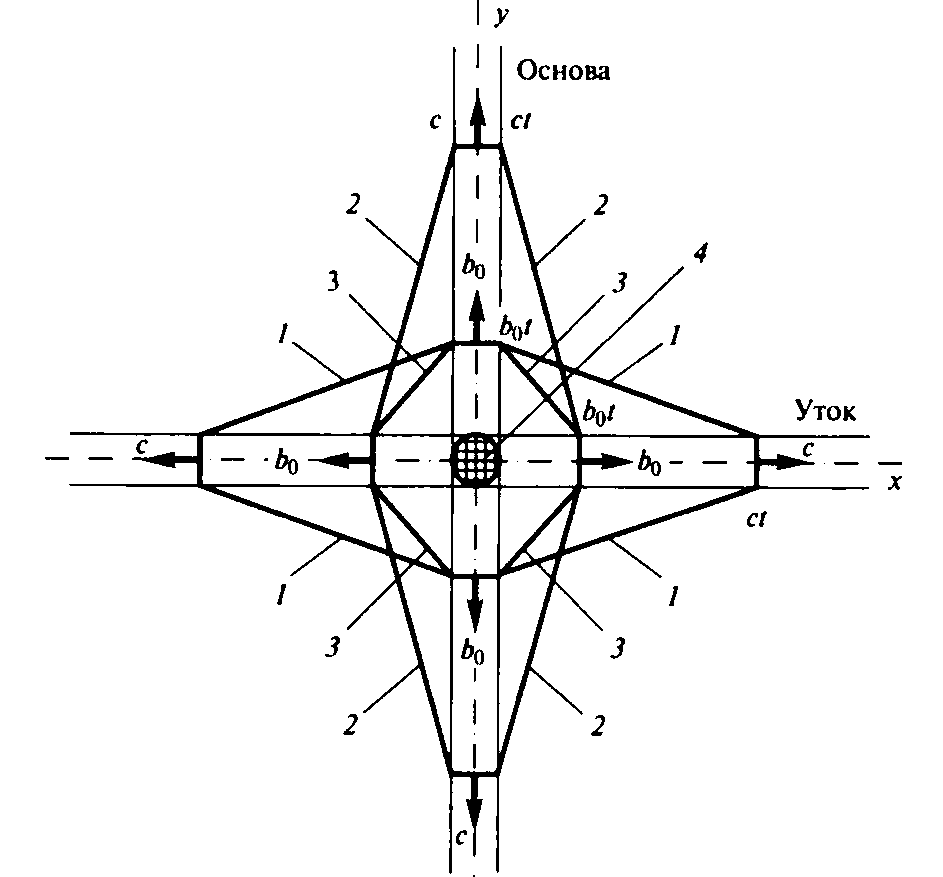
\includegraphics[width=0.5\textwidth]{img/bell_cross_model.png}

    \caption{Пример образца со сквозным пробитием}
    \label{fig:bell-cross-example}
    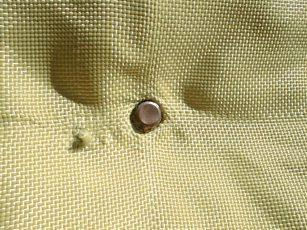
\includegraphics[width=0.5\textwidth]{img/bell_cross_example.png}
\end{figure}

\section{Границы применимости}\label{sec:application}
При применении формул, приведённых выше следует иметь в виду, что они выполняются только при определённых условиях:

\begin{enumerate}
    \item Отсутствие начального натяжения нитей.
Выполняется в силу постановки задачи.
    \item Деформации малы (< 0.1).
Выполняется, так как нити разрушаются при меньших деформациях.
    \item Рассматривается удар с постоянной скоростью по телу бесконечной протяжённости.
\end{enumerate}

Последнее условие имеет смысл рассмотреть отдельно.
При попадании пули в бронежилет её скорость много меньше скорости продольных волн, в нашем случае они сравнимы.
В итоге в задаче появляются следующие особенности:
\begin{enumerate}
    \item Необходимо рассмотреть процесс не до остановки ударника, а до полного пролёта через пакет.
    \item Из-за высокой скорости частиц нет оснований преполагать, что состояние ните подстроится под изменение их скоростей.
\end{enumerate}

На основе данных рассуждений выполняется численное моделирование системы нитей.